\documentclass [t,11pt] {beamer}
%\def\Put(#1,#2)#3{\leavevmode\makebox(0,0){\put(#1,#2){#3}}}

% --------------------------------------------------------------------
% Load packages
\usepackage{ulem}
\usepackage{graphicx}
\usepackage{tikz}
\usetikzlibrary{calc,trees,positioning,arrows,chains,shapes.geometric,%
    decorations.pathreplacing,decorations.pathmorphing,shapes,%
    matrix,shapes.symbols}
\usepackage{listings}
%\lstset{tabsize=2,showspaces=false,showtabs=false,basicstyle=\ttfamily\mdseries\itshape\normalsize}
%for listings:
\usepackage{color}

\definecolor{dkgreen}{rgb}{0,0.6,0}
\definecolor{gray}{rgb}{0.5,0.5,0.5}
\definecolor{mauve}{rgb}{0.58,0,0.82}

\lstset{frame=tb,
  language=R,
  aboveskip=3mm,
  belowskip=3mm,
  showstringspaces=false,
  columns=flexible,
  basicstyle={\small\ttfamily},
  numbers=none,
  numberstyle=\tiny\color{gray},
  keywordstyle=\color{blue},
  commentstyle=\color{dkgreen},
  stringstyle=\color{mauve},
  breaklines=true,
  breakatwhitespace=true,
  tabsize=3
}





% --------------------------------------------------------------------
% Beamer version theme settings
%\usetheme[faculty=sciences,lang=en,rmfont=pmn,logofont=fpi]{leiden}
%\usetheme[faculty=sciences,lang=en]{leiden}
\usetheme[faculty=sciences,lang=en,logofont=fpi]{leiden}

% --------------------------------------------------------------------
\def\liketitle#1{%
{\usebeamerfont{frametitle}\usebeamercolor[fg]{frametitle}%
\begin{flushleft}%
\vspace{-\baselineskip}% Cosmetic correction for space introduced by flushleft
#1\par
\end{flushleft}%
\vspace{-\baselineskip}% Cosmetic correction for space introduced by flushleft
}%
\vspace{0.75\baselineskip}%
}

\setbeamertemplate{navigation symbols} {}

%\usetheme{Singapore}

% Header settings
\def\lecturename{Open Trackers} 
\lecture[Leiden Template]{}{ldn-bmr}
%\lecture[Leiden Template]{}{}
\title{Open Trackers for (Open) Science} 
%\subtitle{Template to generate Leiden-style slides with LaTeX}
\author {Daniela Gawehns, Froscon 2020}
\date{}
%\institute{Universiteit Leiden}
\subject{Lecture: \lecturename}



\begin{document}


\maketitle


\begin{frame}
\frametitle{Outline}
\tableofcontents
\end{frame}

\begin {frame} {Wrist-worn }
\center
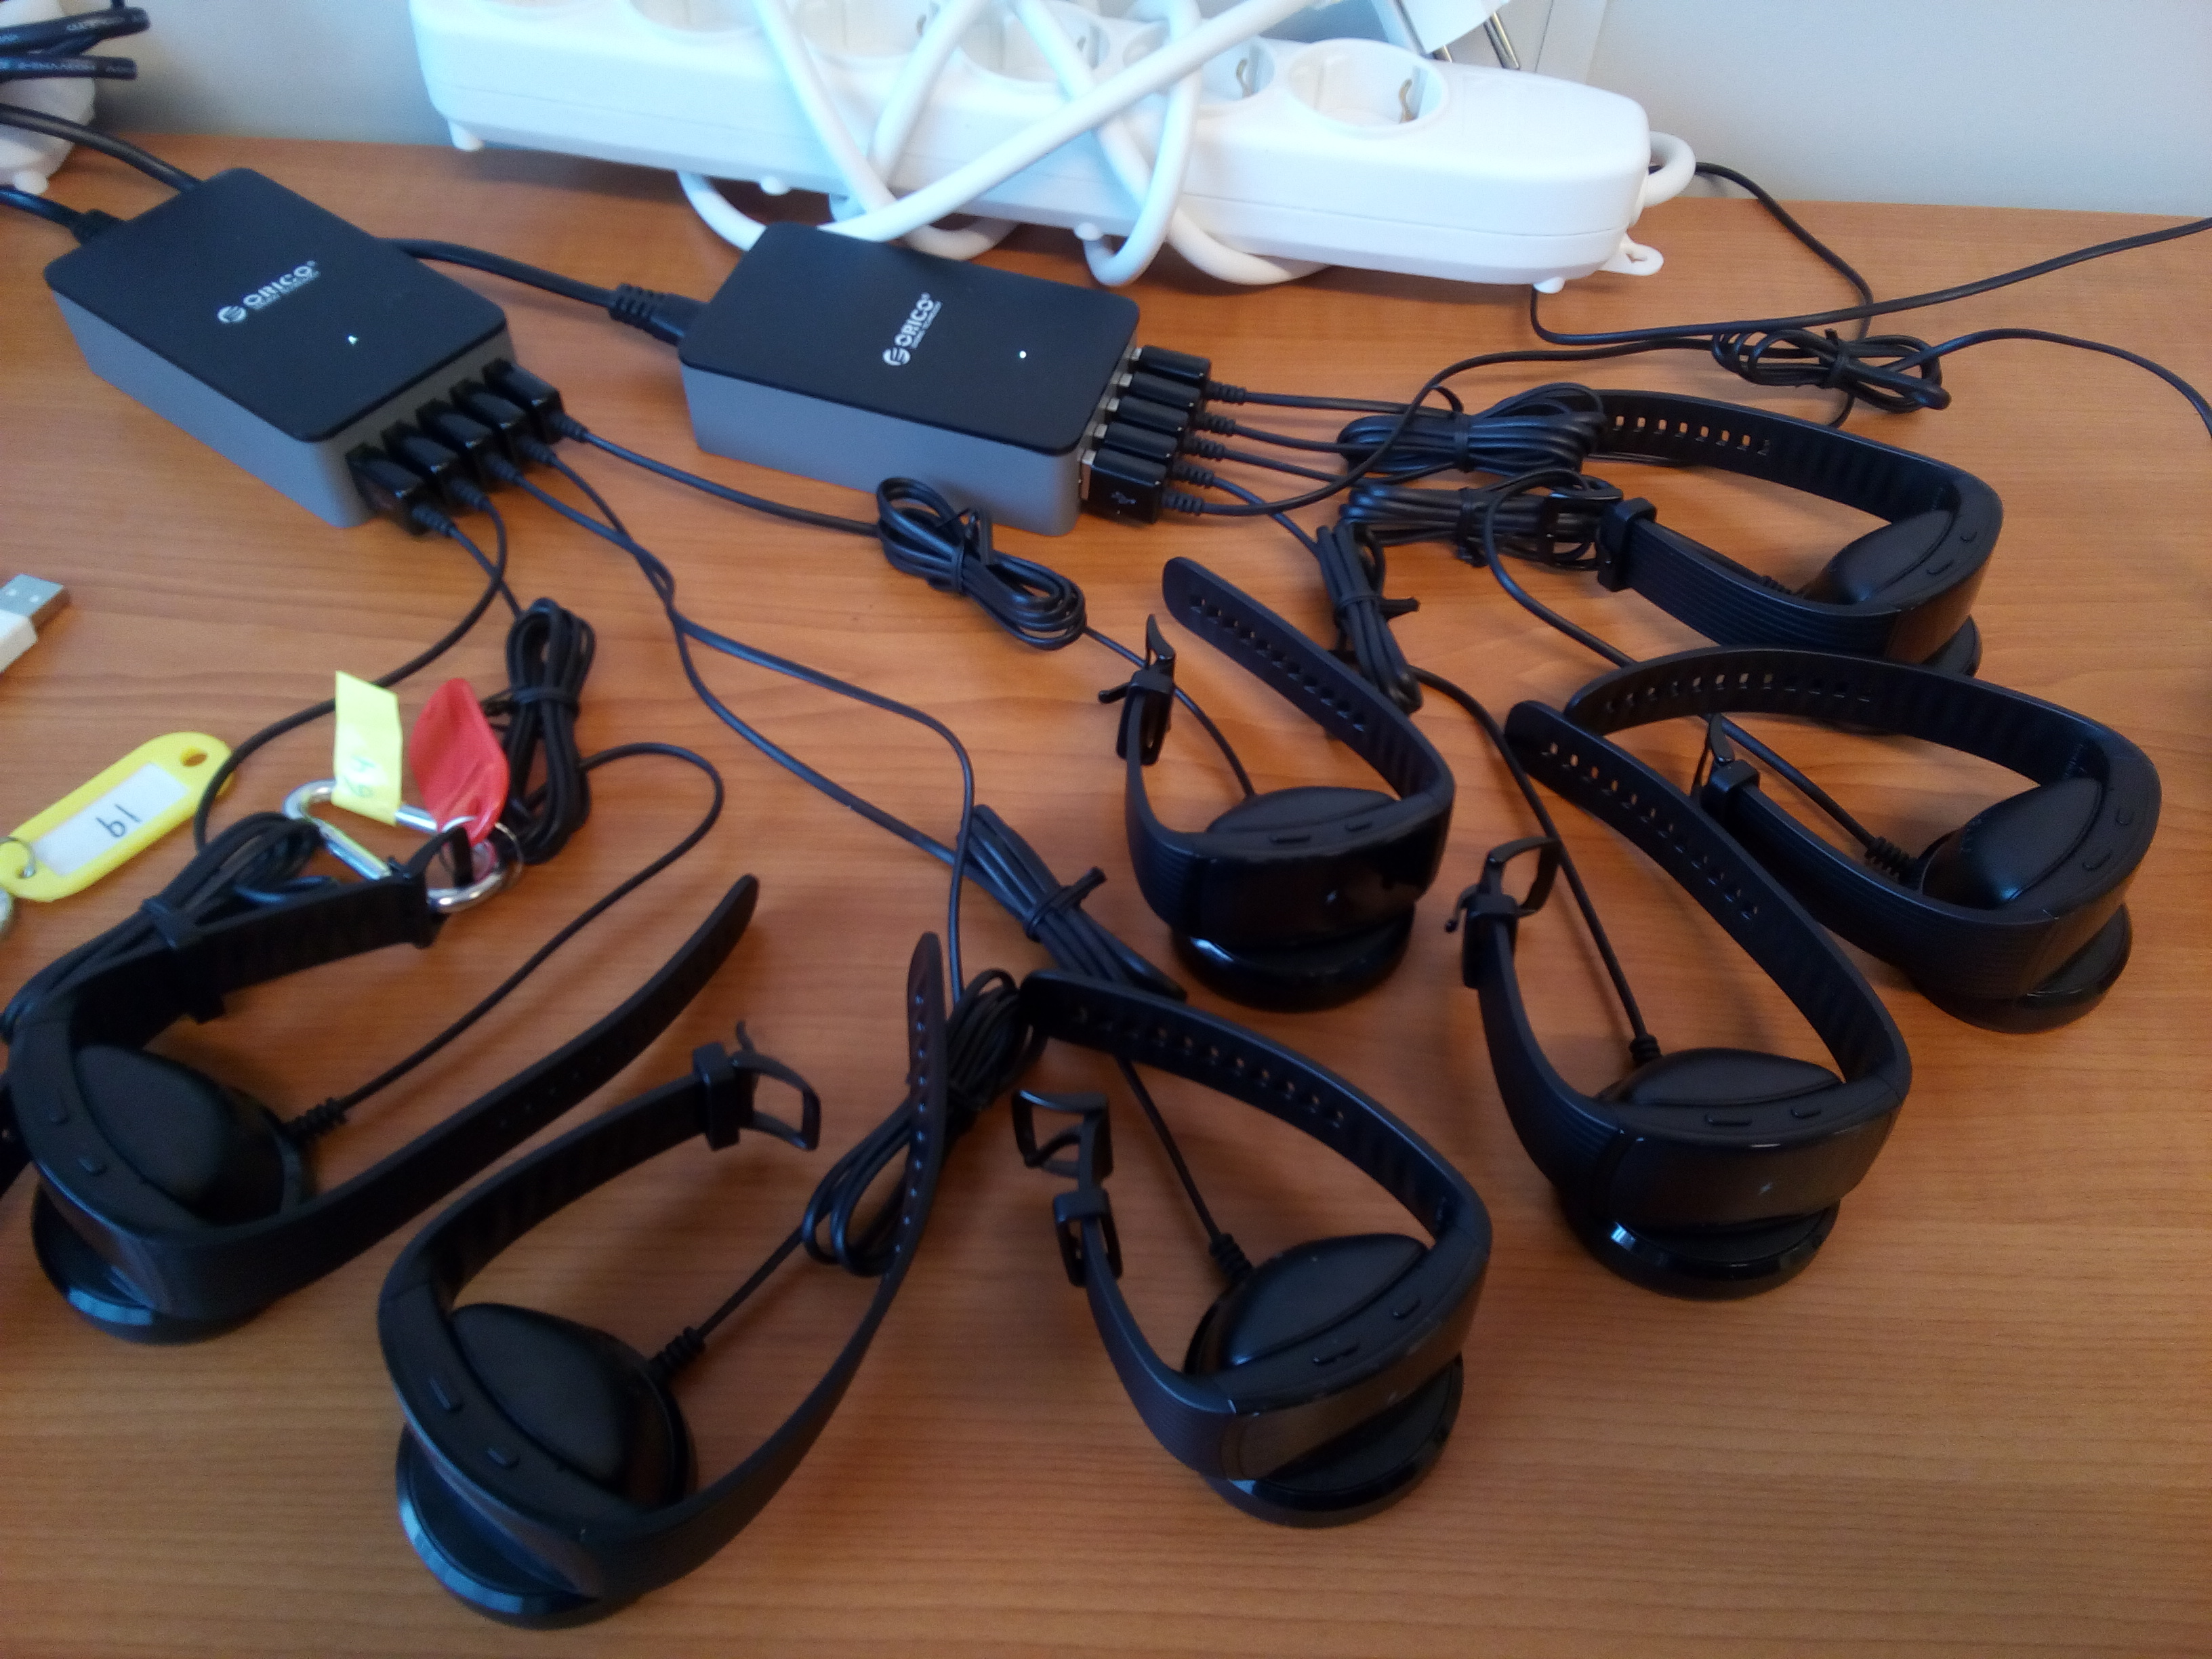
\includegraphics[width=80mm]{img/trackers}

%Twins, age 8, go to primary school
% Come home with a letter "Invitation to participate" 
% Study on how children play and what they like most about their school
% There will be a few surveys, researchers will take notes and observe children and the kids will be outfitted with a smart watch for a week during school hours. The researchers will record with the watches the locations, interactions and activity of the children.


\end {frame}



\section {Using Activity Trackers for Research}

\subsection {Participating in Research}
\begin {frame} {Three Personas I}
Persona I : Mark
\center

\includegraphics[width=30mm]{img/IconOne}

%Twins, age 8, go to primary school
% Come home with a letter "Invitation to participate" 
% Study on how children play and what they like most about their school
% There will be a few surveys, researchers will take notes and observe children and the kids will be outfitted with a smart watch for a week during school hours. The researchers will record with the watches the locations, interactions and activity of the children.


\end {frame}

%%%%%%%%%%%%%%%

\begin {frame} {Three Personas II}
Persona II : Janine
\center

\includegraphics[width=50mm]{img/IconTwo}

%Just out of prison, it is not important to know why she served prison time
%Has a history of criminal conduct, being in and out of specialized psychiatric care, meeting with social workers and in and out of prison/ juvenile detention
%With her coach, she has found out which triggers make her more likely to spiral back into criminal behavior.Her coach suggest to participate in a study, where she will be wearing a smartwatch that is recording all kinds of activities, and notifying her coach or a person of confidence when these triggers are encountered. In her case not getting out of bed for days on end and contacting a handful of people that are linked to unlawful behavior. 

\end {frame}

%%%%%%%%%%%%%%%

\begin {frame} {Three Personas III}
Persona III : Karla 
\center

\includegraphics[width=50mm]{img/IconThree}

%Karl's mother is in a nursing home as she cannot live at home anymore because of her dementia
%Invitation to participate in a study where researchers want to observe the activities at the nursing home to find out how much residents are moving and are physically active. The researchers will also be using smartwatches to record movement and location of the residents. Karl can give consent to either: only observations and surveys, observations, surveys and smartwatch during the day or all of the above and smartwatch at night, too. 
%

\end {frame}


\subsection {Activity: Alarm bells}
%%%%%%%%%%%%%%%

\begin {frame} {Three Personas}

%Three Icons 

\includegraphics[width=30mm]{img/IconOne}
\includegraphics[width=30mm]{img/IconTwo}
\includegraphics[width=30mm]{img/IconThree}
%Link to mentimeter or other poll option

\pause 
\hspace {1cm}

https://hackmd.io/@DGawehns/rylqLQpMv/edit

%Imagine you were a parent and enrolled your child in a study, you enrolled yourself in a therapeutic program or were asked to enroll your parent living with dementia: Which alarm bells will this trigger and which problems do you see?

\end {frame}

%%%%%%%%%%%%%%%


%%%%%%%%%%%%%%
\begin {frame} {Summary Feedback}

%how to summarize? 


%add Design: durable, "normal looking"/ stigma avoiding. Data Privacy: full control over sharing data

\end {frame}

%%%%%%%%%%%%%%%



\subsection {Conducting Research}


%%% From a researcher's perspective: what makes those trackers attractive? 

%%%%%%%%%%%%%%
\begin {frame}{The Why }

What makes those activity trackers so attractive?

\begin {itemize}
    \item tracking of activity, heart rate, location, interactions, momentary emotional assessment
    \item passively, (almost) non-intrusive
    \item longitudinal studies (several weeks)
    \item real life data
\end {itemize}

\end{frame}
%%%%%%%%%%%%%%


%%%%%%%


%Speakernotes:

%At exodus, ex detainees get coaching to build a new life after prison. This includes making plans and monitoring that coachees stay out of prison.

%This is traditionally done with personal sessions and via phone calls.

%Wearables could help clients at exodus to gain more insights about their own behavior and give them feedback about their behavior. Depending on the clients wishes, coachees could have their coach call them if they stayed insight for too long and fear that this triggers a spiral of depression and drug abuse. Or, going even further, the wearable could monitor which calls are made from the mobile phone and if a set of numbers is or is not called, the coach gets a message and reminds the coachee to call their support system or asks what made them get in touch with criminal circles again.


%%%%%%%%%%%%%%
\begin {frame} {Summary of Use Cases}
%include overview/ schema with Data Collection and Case Study
\center
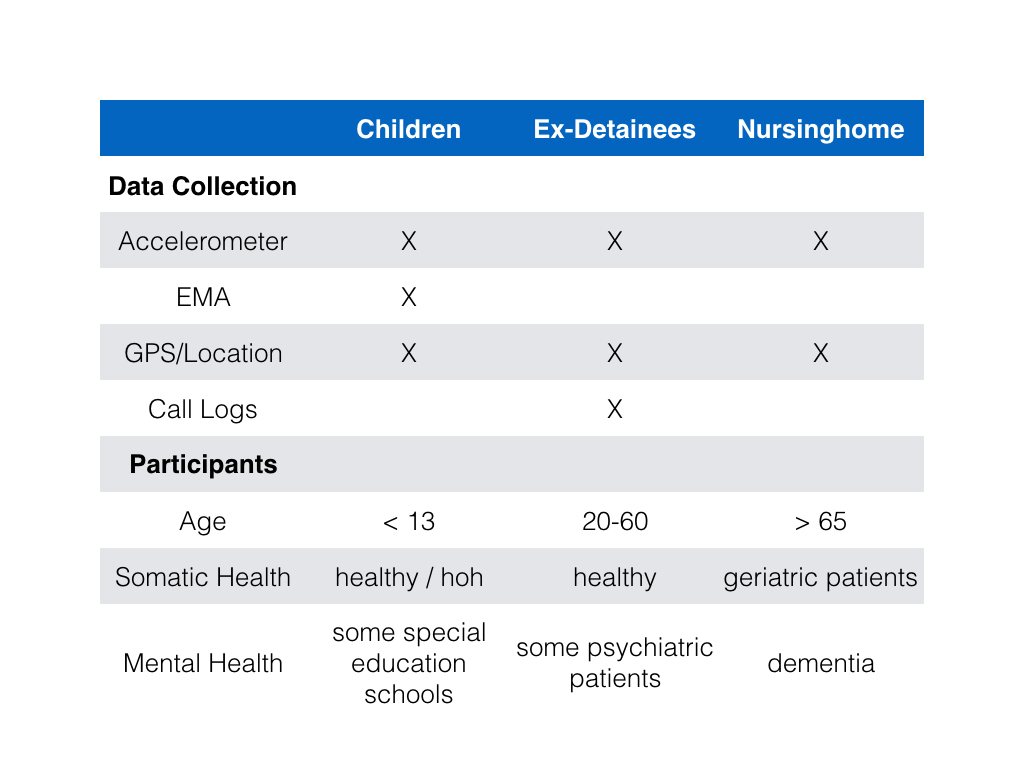
\includegraphics[width=80mm]{img/OverviewUsecases}

\end {frame}

%%%%%%%%%%%%%%



%%%%%%%%%%%%%%
\section {Which hardware and software options exist?}

%%%%%%%%%%%
\begin {frame}{The How - Balancing Acts}

\center
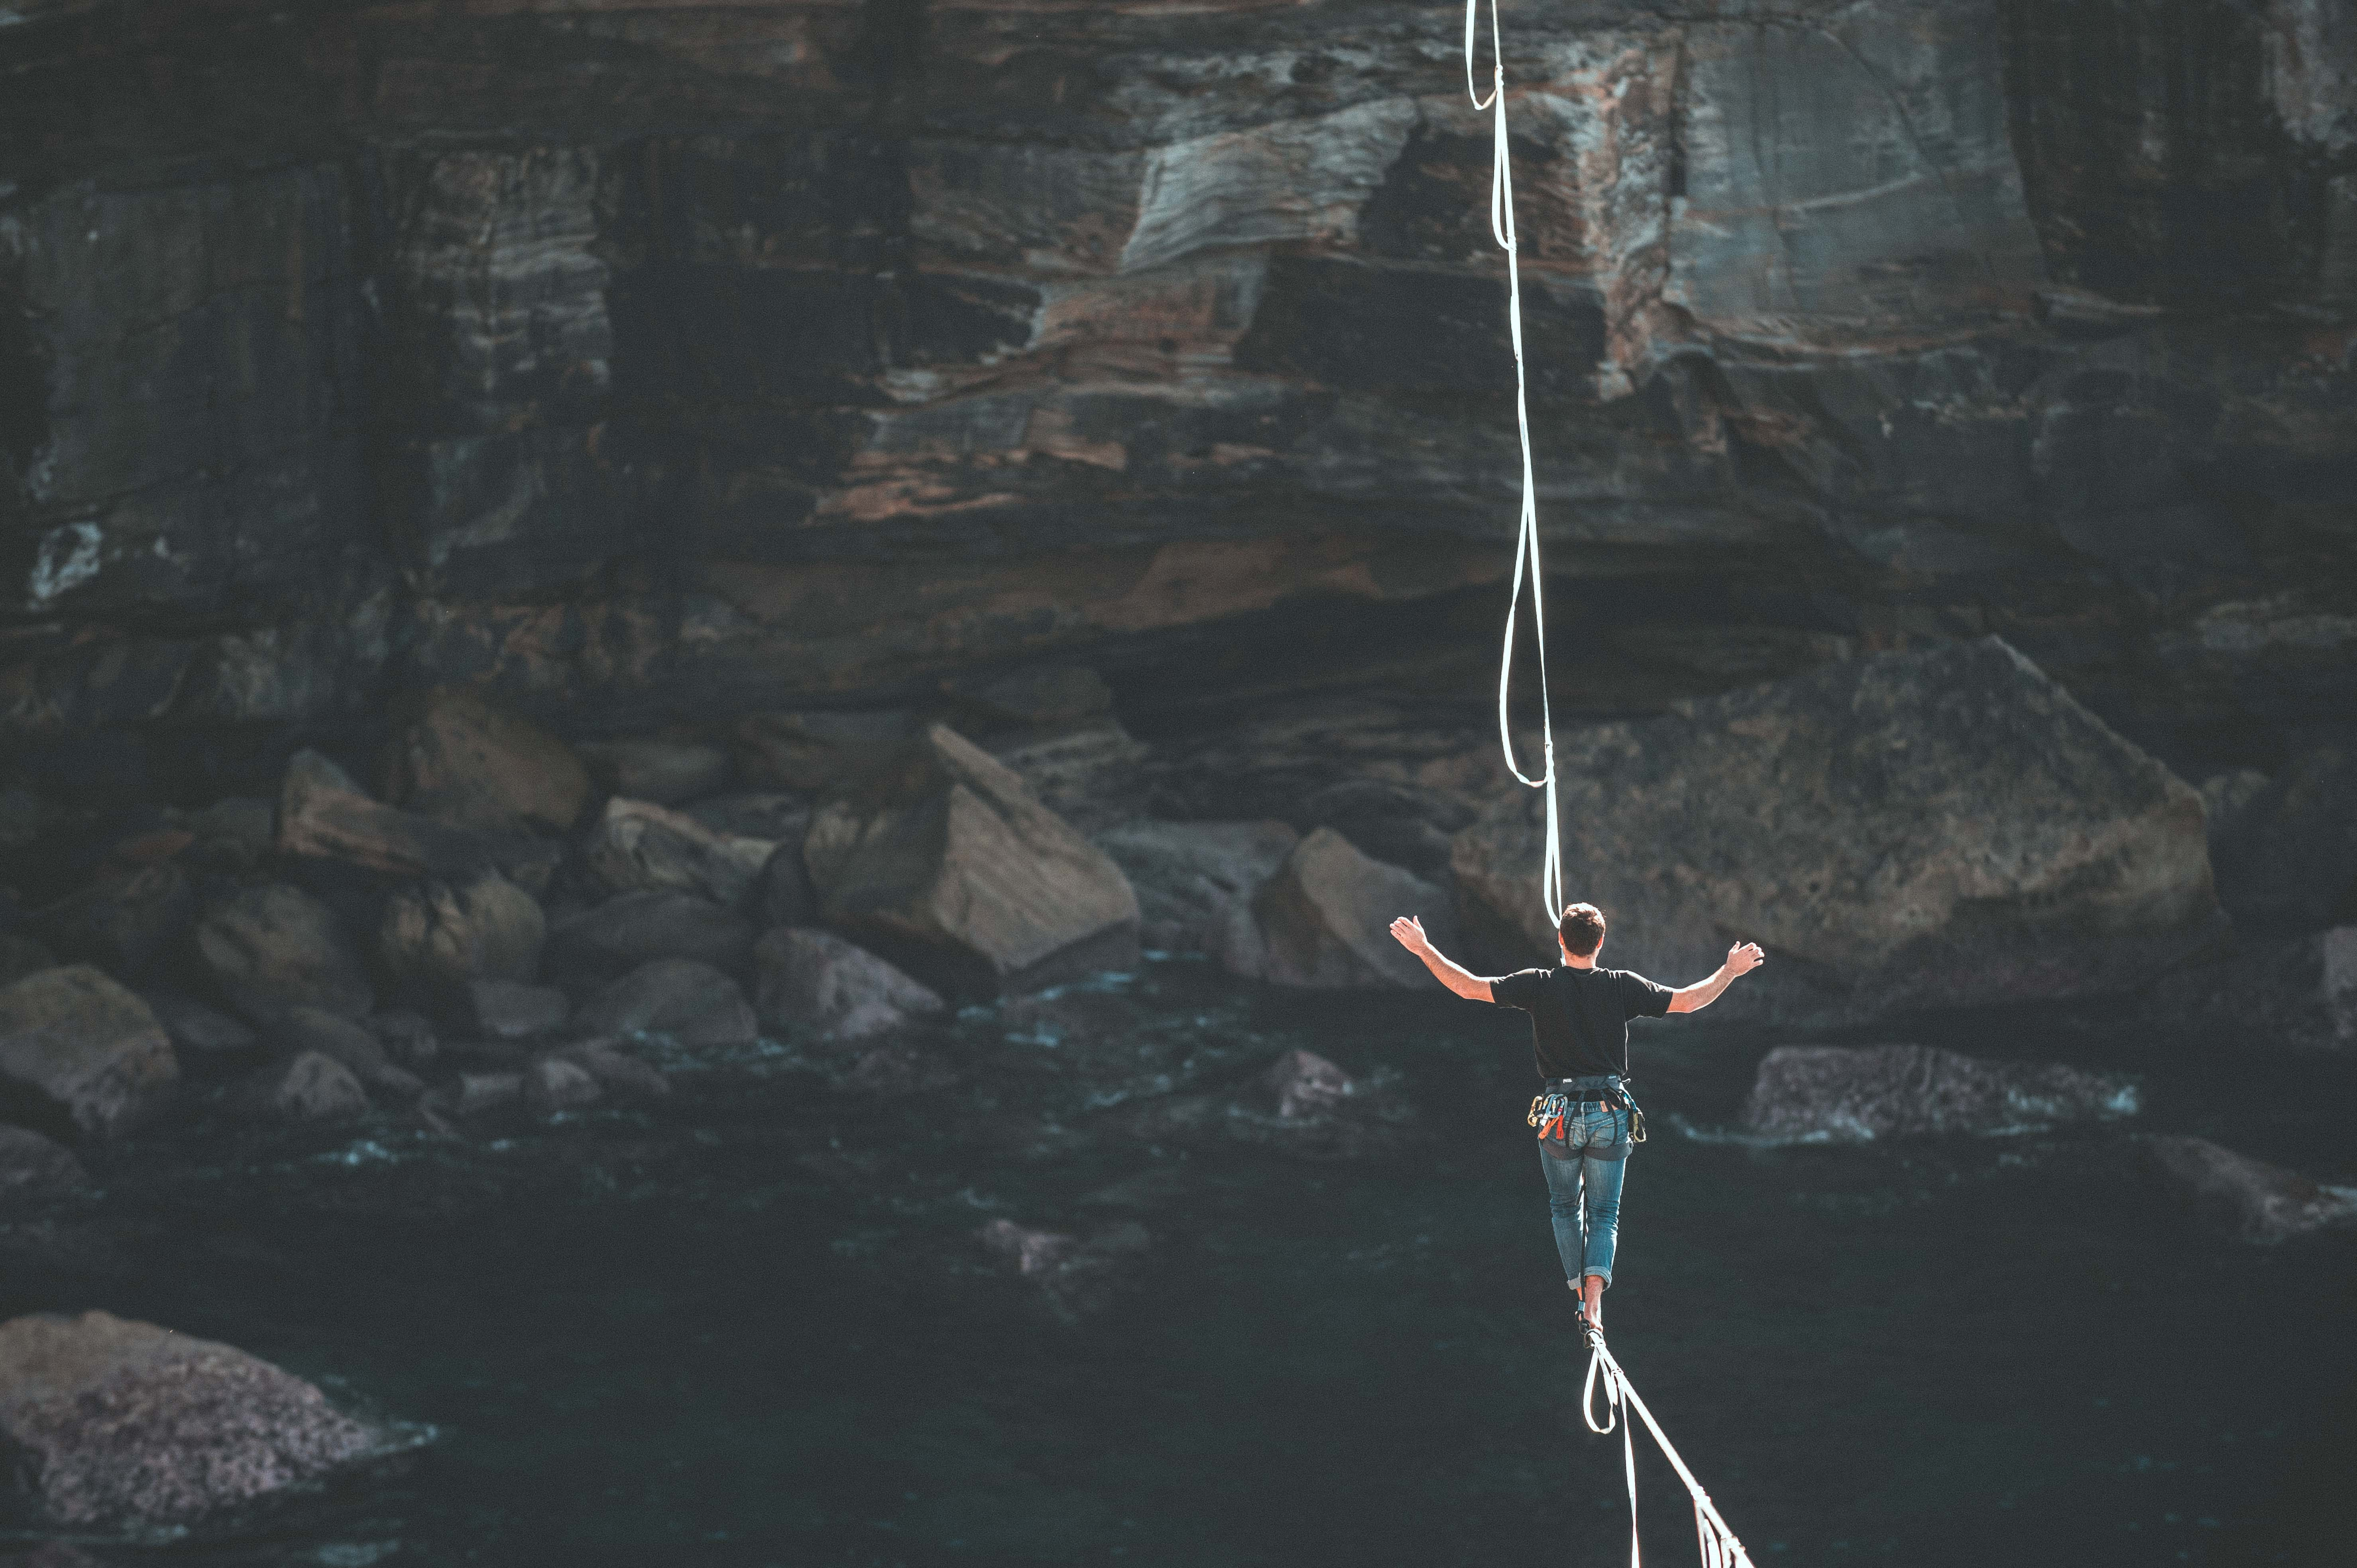
\includegraphics[width=60mm]{img/balance}

\vspace {1.5cm}

{\fontsize{5}{6}\selectfont Photo by  Loic Leray on Unsplash} 


%Data Quality - Scalability
%Interoperability - Utility

%Balancing act btw a lot of issues and factors! Looking at why ppl are using closed systems and looking at the advantages those systems promise is useful when designing or searching for an open system - it helps you design a useful system

\end {frame}
%%%%%%%%%%%


%%%%%%%%%%%

%- Data Privacy Solutions - only for offline/closed system devices - lab setting only
%- Use research platforms by Garmin or fitbit to access data
%- Using customer grade products and code the software yourself

\begin {frame}{The How - Current Hardware Options}
\begin {columns}

\begin {column}{0.5\textwidth}
\textbf{Medical Research Devices}

\includegraphics[width=30mm]{img/MedDevices}

\begin {itemize}
\item Shimmer
\item Actigraph
\item Empatica
\item ... and many more
\end {itemize}

\end {column}

\pause

\begin {column}{0.5\textwidth}

%choosing a platform not just a piece of hardware, but a combination of hardware, firmware, operating system and software stack -- all in a bundle and often, you wont be able to take it apart

\textbf {Consumer Grade Devices}

\includegraphics[width=30mm]{img/ConsDevices}

\begin {itemize}
\item Apple Watch
\item fitbit  
\item Garmin 
\item Android Watches
\item Tizen 
\item astroid %- virtual machine on android OS
\end {itemize}

\end {column}
\end {columns}

\end{frame}

%%%%%%%%%%%%





%%%%%%%%%%%


\begin {frame}{The How - Apple Watch}

\begin {itemize}
\item Partner with the Apple Research App %props totally not possible unless you'r Harvard or MIT
\item Researchkit and Carekit frameworks 
\pause
	\begin {itemize}
	\item access health data, access to "tasks" and their outcomes
	\item bring your own data storage (?!)
	\item locked into what the frameworks allow (e.g., no background data collection)
	\item locked into Apple Watches
	\end {itemize}
%are open source, so no involvement by apple on what you are doing (?)
%you can bring your own backend and manage data storage yourself (!?) %locked in to use apple watches, locked in to use the functions that the frameworks supply %for example background data collection might not be possible
\pause
\item Apple Watch App (e.g. Apple Watch SensorLog) 
	\begin {itemize}
	\item locked in by certification/ app store process 
	\item locked in to Apple Watches
	\end {itemize}

\end {itemize}

\end {frame}

%%%%%%%%%%%%


%https://www.researchandcare.org

%Investigator Support Program to get watches for your study

%Researchkit: Tasks (e.g., Stroop Task, Walk as quick as you can)
%		     No background data collection
		     
%Healthkit: Access Health data via this kit

%CoreMotion: "Core Motion reports motion- and environment-related data from the onboard hardware of iOS devices, including from the accelerometers and gyroscopes, and from the pedometer, magnetometer, and barometer."

%--> open questions: 
%will data be sent only btw app and researcher?
%which temporal granularity of raw sensor data output is achievable?
%what is the reliability/ validity of the in-built cognitive assessments?


%General: Investigator Support Pilot and Apple watch limited grant program

%		http://researchkit.org
%		https://github.com/researchkit/researchkit
%		https://developer.apple.com/videos/play/wwdc2019/217/
%		docs: http://researchkit.org/docs/docs/Overview/GuideOverview.html
		 
%		 Tasks: seven categories: motor activities, fitness, cognition, speech, hearing, hand 				dexterity, and vision
%		 All from Clinical Neuropsychology - Cognitive and fitness testing activities
%		 the clinician in me asks: are those validated tests? Validated againsts paper-pen tests or lab tests that those are based on 
		 
%		 It might be returning the raw accelerometer information collected during those tasks (???)
%		 You can also design your own test (?)
		 
		
%		ResearchKit framework currently doesnt include:

%Background sensor data collection. APIs like HealthKit and CoreMotion on iOS already support this.
%Secure communication mechanisms between your app and your server; you will need to provide this.
%The ability to schedule surveys and active tasks for your participants.
%A defined data format for how the ResearchKit framework structured data is serialized. All the ResearchKit framework objects conform to the NSSecureCoding protocol, and sample code exists protocol, and sample code exists outside the framework for serializing objects to JSON.

%Healthkit - needed to access users health data and information: 
%		demographics, workout information (?) but where is the sensor data?

%CoreMotion - 
%docs: https://developer.apple.com/documentation/coremotion
%Core Motion reports motion- and environment-related data from the onboard hardware of iOS devices, including from the accelerometers and gyroscopes, and from the pedometer, magnetometer, and barometer.
%	Accelerometer, 
%	Gyroscope,
%	Magnetometer
%	Altitude
%	Pedometer,

%Looking into Accelerometer: value of recording interval seems to depend on hardware? ??
%Interesting finding: they have a function and objects to monitor movement disorders, namely tremors

%%%%%%%%%

\begin {frame}{The How - Fitbit}

\begin{itemize}
\item Use Fitabase  %a company providing research support
\item Use web API %- extract customer data per participant 
	\begin{itemize}
	\item Companion Application to Watch Application file transfer  %can this be done via a private network? fetch API seems to allow this - at least that's what the docs say
	\item locked in certification  %private apps need to go through publishing process? you might be able to play the system and have several dev accounts and associated dev watches with it - only possible on some, not all watches: Fitbit Versa, Versa Lite, Versa 2, and Ionic.
	\end{itemize}
\item Use bulk download via fitbit account %doable for small studies - locked in to what fitbit grants you access to via the companion application
\end {itemize}

\end {frame}
%https://healthsolutions.fitbit.com/researchers/
%https://healthsolutions.fitbit.com/researchers/faqs/ %but the accelerometer API DOES give you access to raw accelerometer data??
%https://www.fitabase.com - company providing researchsupport

%broad product lineup with devices that track a variety of metrics, including step count, floors climbed, distance, calories burned, active minutes, sleep time and stages, and heart rate

%Either summary data per account: 
%https://help.fitbit.com/articles/en_US/Help_article/1133.htm

%or via web API for accessing data from Fitbit devices and anyone can develop an application to access data from a device - in higher temporal resolution, including GPS data (Heart Rate, Sleep, Activity Patterns) --> Intraday support can extend the detail-level response to include 1min and 15min for Activity, and 1sec and 1min for Heart Rate
%on researchers/faq:
%Can I access raw accelerometer (or other sensor) data?
%No, this data cannot be accessed. See above for more information on the data you can access and how you can do so.

%--> open questions: 
%Is an offline export of the data possible and supported?
%(i.e. not via web API)
%General  question about the black boxes converting sensor data into activity types or counted steps

%%%%%%%%%%%%%%%%%



%%%%%%%%%				
\begin {frame}{The How - Garmin}		

%https://www.fitabase.com - company providing researchsupport
%https://www.fitabase.com/how-it-works/faq/
%https://www.fitabase.com/resources/knowledge-base/learn-about-fitbit-data/data-resolutions/
%granularity of data available

\begin{itemize}
\item Use Fitabase - a company providing research support
\item Use the Health API 
\item Use the Health SDK 
\end {itemize}

%https://developer.garmin.com/health-api/overview/ 
%Health API and Health SDK

%Health SDK allows custom recording of Heart Rate, Activity Types - and most probably also accelerometer and gyroscope data (but no confirmation or link information for any of this)


%Health API gives access to a range of data collected, activity types, sleep, heart rate; I am pretty sure that extraction of raw accelerometer data is not possible via this 

\end {frame}



%%%%%%%%%%%%%%%%%

\begin {frame}{The How - Using Big Tech}

\begin {itemize}
\item Availability, Scalability % for population studies - large trends 
	\begin {itemize}
	\item https://corona-datenspende.de %it is an app to read data from health and fitness apps - i.e. not to read info directly from the watches
	\end {itemize}
\pause
\item Design Choice - Working with participants or patients
\end {itemize}

%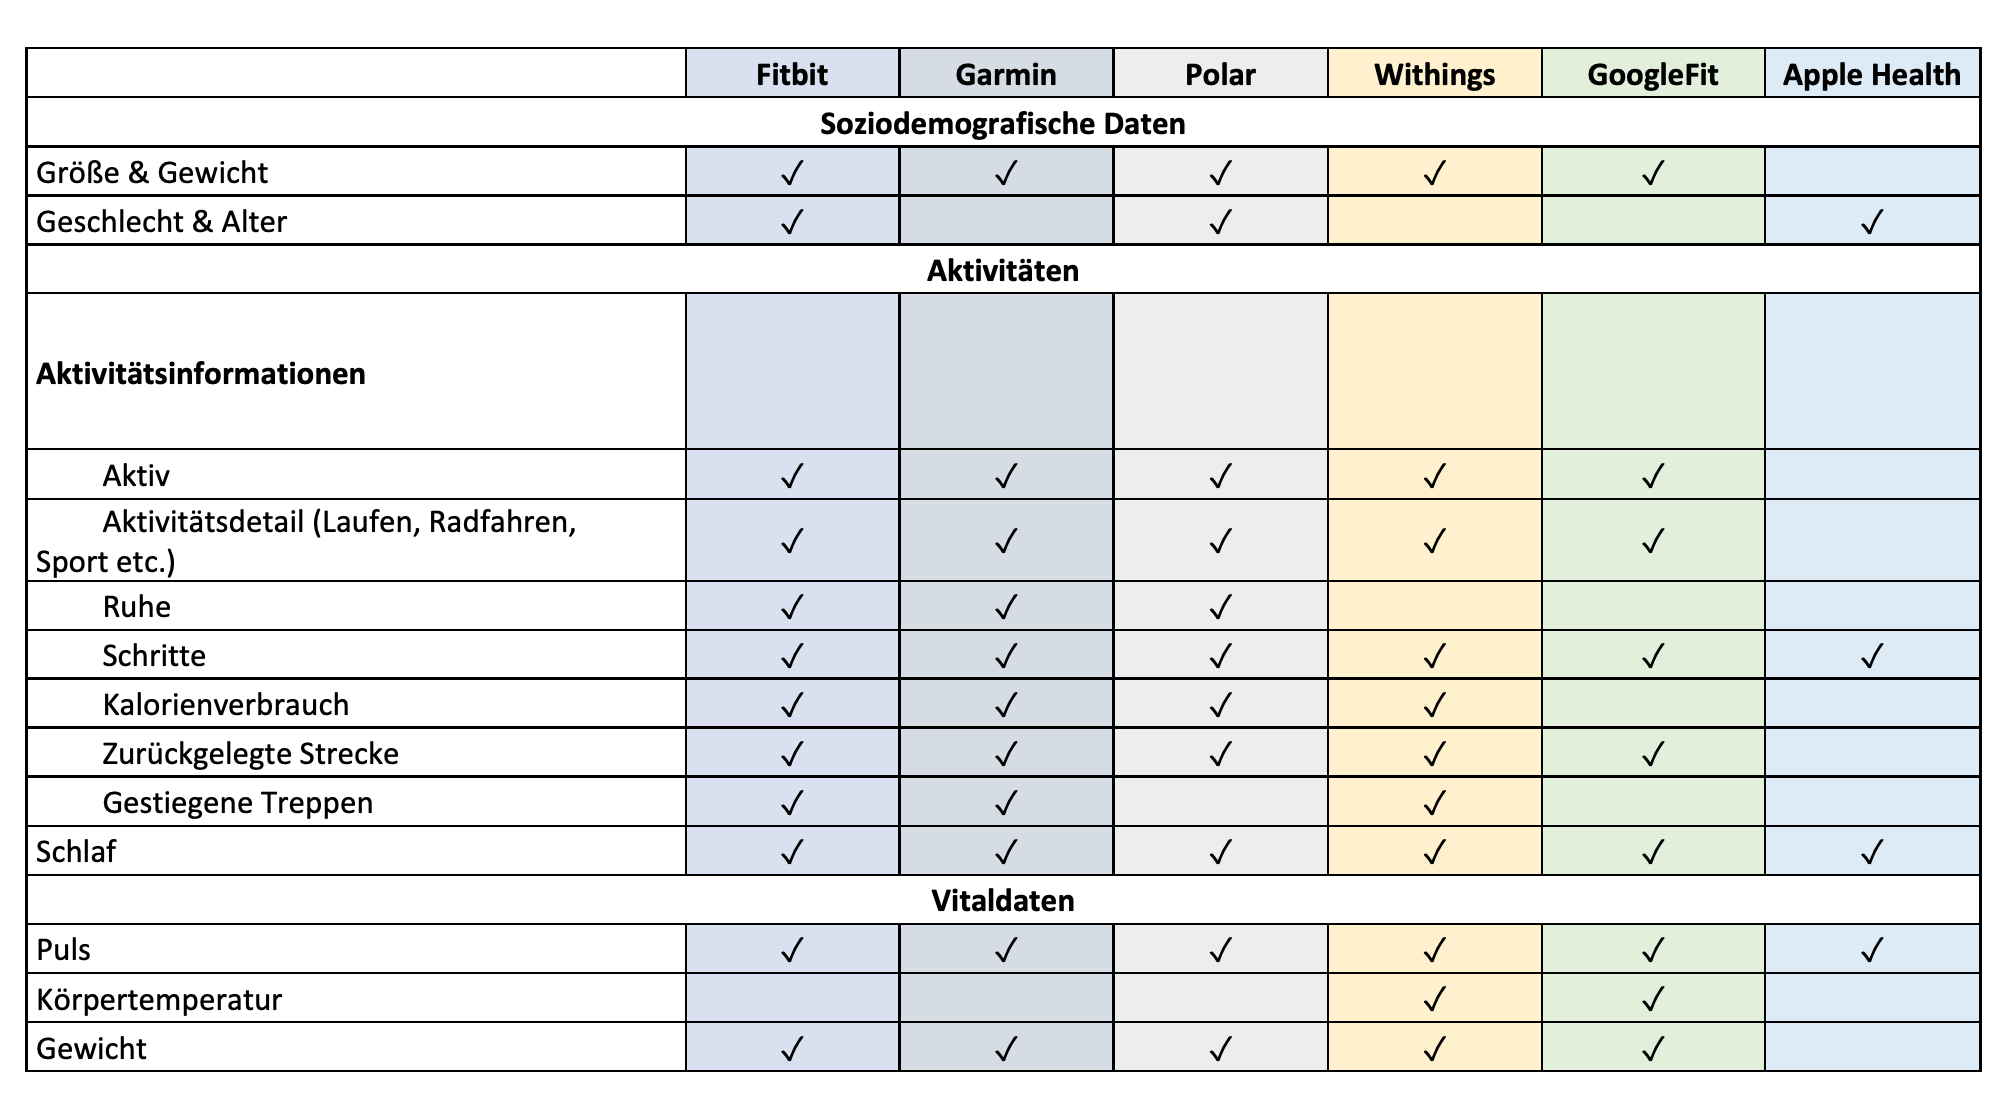
\includegraphics[width=30mm]{img/datadonation}


\end {frame}
%%%%%%%%%%%%%%%%%%%%%%%%%%

%%%%%%%%%%%%%%%%%

\begin {frame}{The How - Choices }

"To \textbf{enhance acceptability} and minimize user burden and stigma, widely available consumer-oriented technologies were therefore considered. The user groups favored the wrist-worn Fitbit Charge HR (Fitbit Inc, San Francisco) due to its \textbf{appearance as a lifestyle device} that is acceptable to both younger and older users and the \textbf{ability to view metrics} relating to sleep and activity via the Fitbit app."

\hspace {1.5 cm}

\small{Meyer N., et al (2018): Capturing Rest-Activity Profiles in Schizophrenia Using Wearable and Mobile Technologies: Development, Implementation, Feasibility, and Acceptability of a Remote Monitoring Platform}

\end {frame}
%%%%%%%%%%%%%%%%%%%%%%%%%%


\begin {frame}{The How - Choices }
"Do these devices, therefore, have a role as tools for clinical prediction?\\
We suggest that they do, \textbf{depending on the question being asked [58]}. Our goal is not to draw conclusions about sleep parameters (eg, total sleep time, sleep efficiency) per se, for which the use of unvalidated devices would be inappropriate. Rather, our \textbf{objective is to ask whether changes in longitudinal rest-activity patterns} at the within-person level, captured using wearable device and smartphone sensors, \textbf{predict deterioration} in clinical status."

\end {frame}
%%%%%%%%%%%%%%%%%%%%%%%%%%



\begin {frame} {Locked - in: corona-datenspende}

%Apart from being locked-in on one set of hardware or one software release and depending on externals to be able to run your app, also the collected variables are "locked -in"

% insert screenshot corona datenspende app 
\center
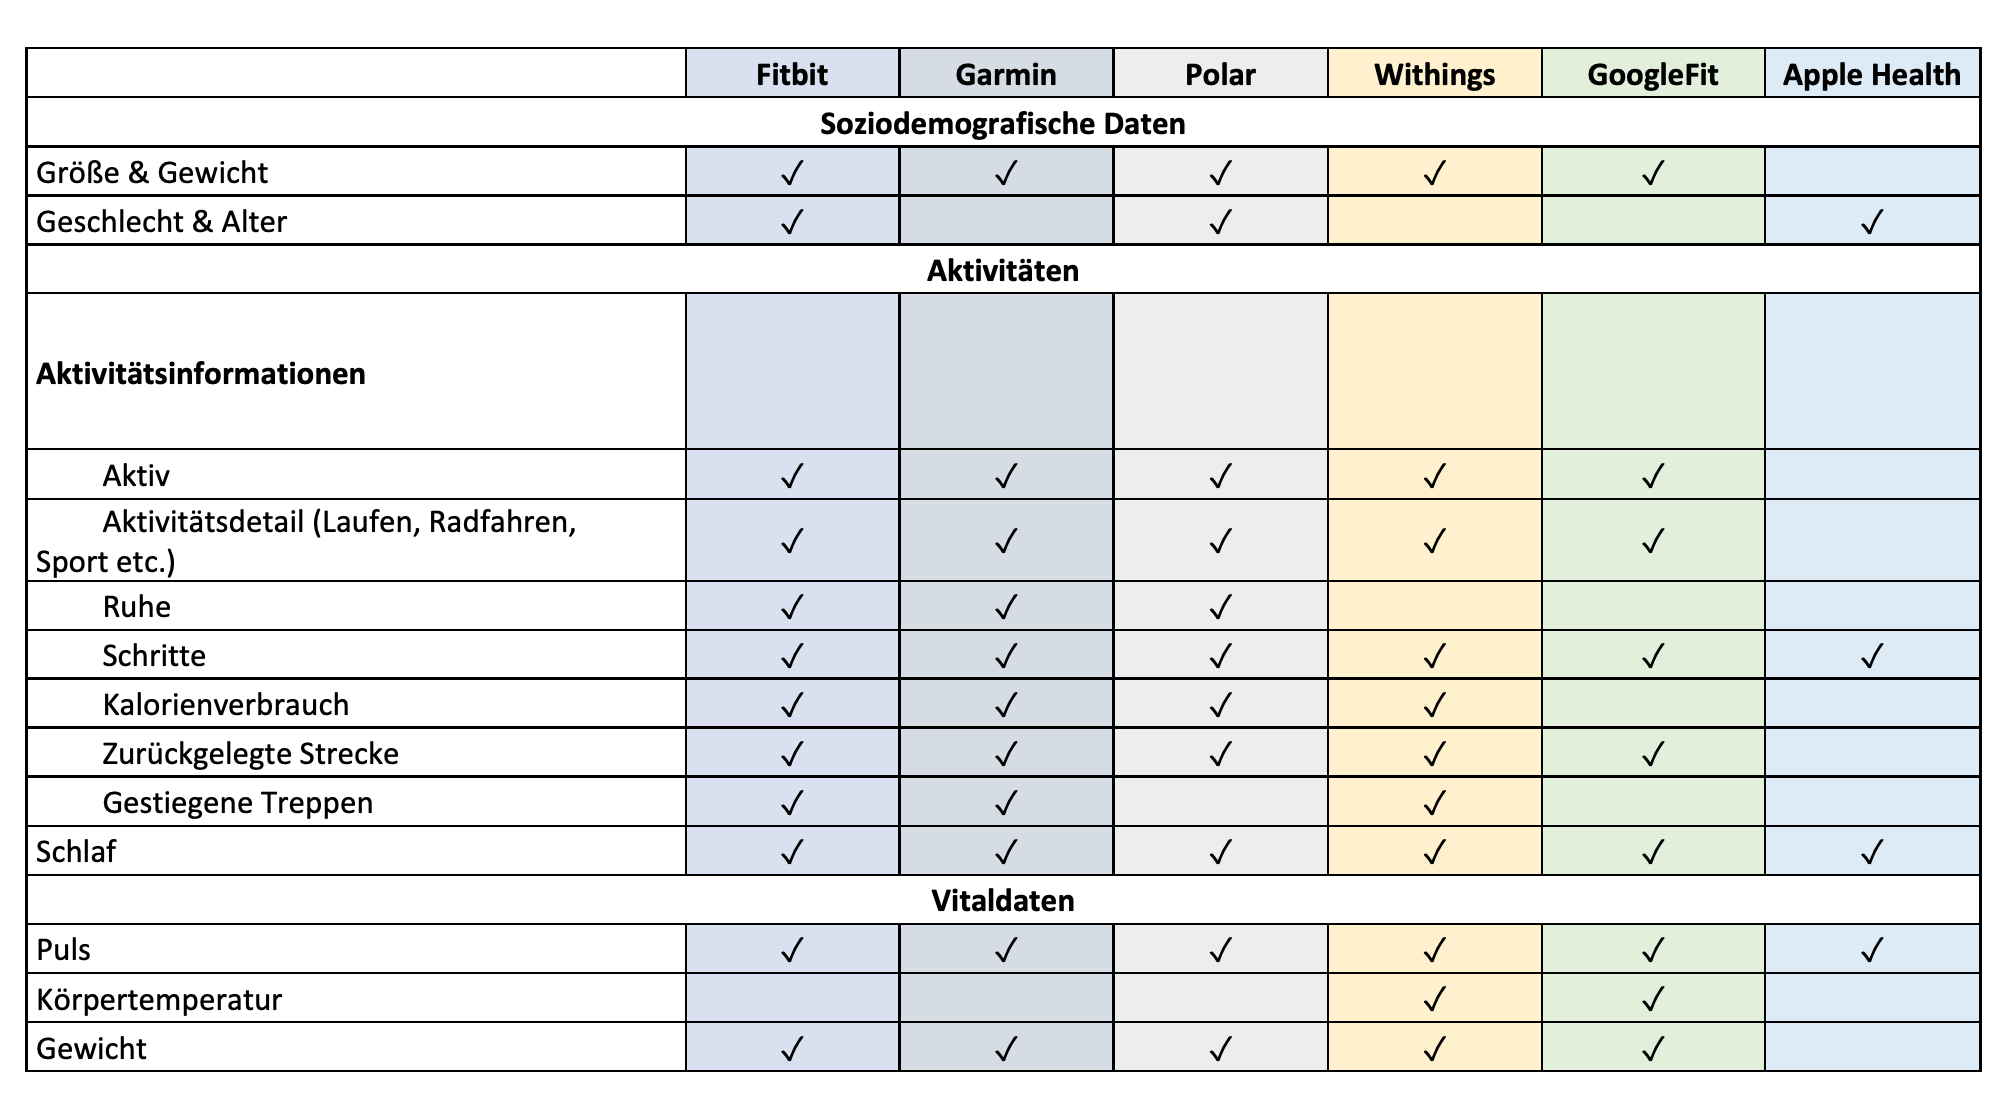
\includegraphics[width=100mm]{img/datadonation}

% these all look to me like derivatives of accelerometer data --- where you have accelerometer data + black box == output

% What does this do for your conclusions??

% What does this do on the long run for your product, intervention, generalization and hypothesis generation and theory building?

% aim of datenspende: die Ausbreitung der Infektionen einsch�tzen zu k�nnen - i.e. no individual prediction of how you are doing, but general trends; they use postal code for approximation of where people are - more or less 

\end {frame}


%%%%%%%%%%%%%%%%%%%%
\begin {frame}{The How - Summary}

Summary: We have solutions for: 

\begin {itemize}
\item Lab Studies \\ \pause bulky, precision technology and access to the raw data
\pause 
\item Big Data Studies \\ \pause  wide spread use of consumer grade devices and access to summary statistics
\pause 
\item Real life Data Collection \\ \pause  if the data supplied by platforms are in accordance with what you want to achieve

\end {itemize}

%(Long term) studies looking to 
%	explore data 
%	explain systems 
%	test hypotheses
%	generate theories and hypotheses


%Technology to be used in therapy and coaching that allows for 
%	personalized therapy
	

%And all of that while having full control over data shared and adhering to the principle of minimal data collection. 

\end {frame}	


%%%%%%%%%%%%%

\begin {frame}{The How - Case Studies}

\center
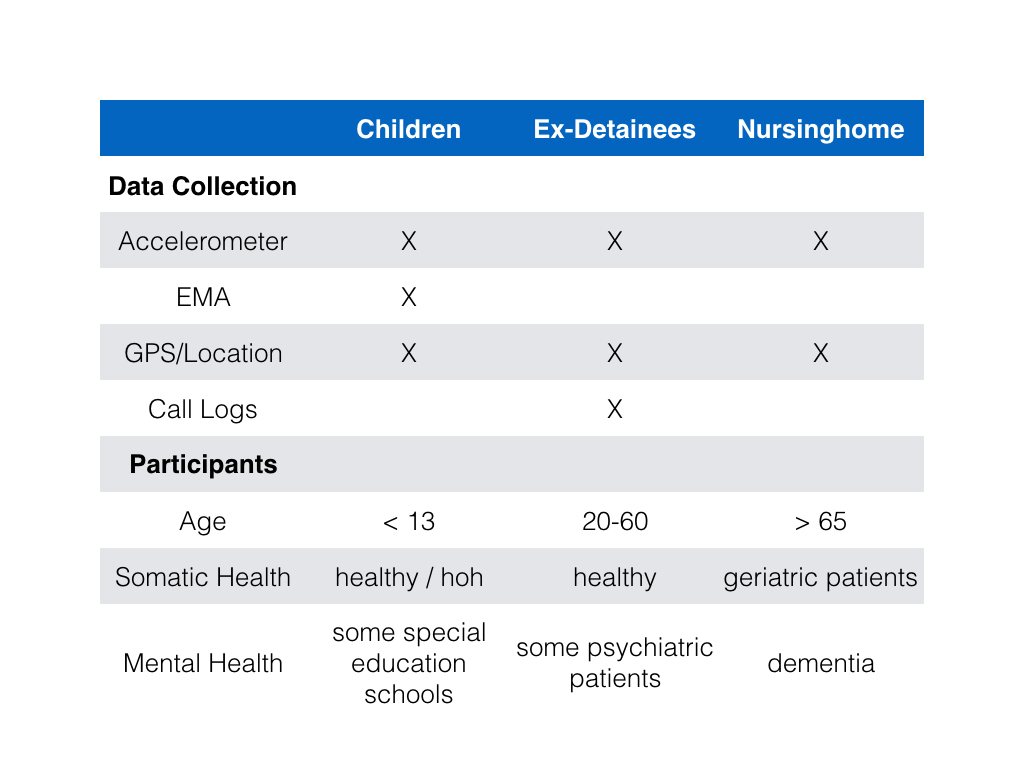
\includegraphics[width=80mm]{img/OverviewUsecases}

%% these are not Lab Studies
%% these are not Big Data Studies
%% these are Real Life Data Collection Studies -- But is the data that we can extract good enough?? 

\end {frame}

%%%%%%%%%%%%%%

%%%%%%%%%%%%%

\begin {frame}{The How - Case Studies}

\center
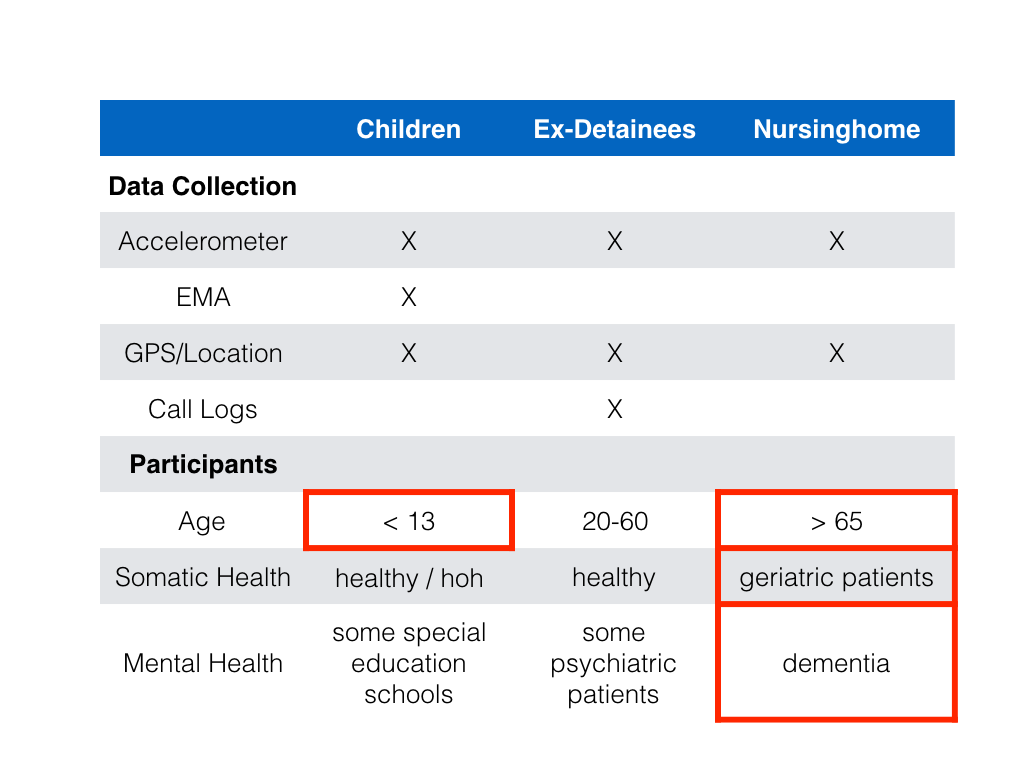
\includegraphics[width=80mm]{img/OverviewUsecasesModels}



%% these are not Lab Studies
%% these are not Big Data Studies
%% these are Real Life Data Collection Studies -- But is the data that we can extract good enough?? 

\end {frame}

%%%%%%%%%%%%%%

\begin {frame}{The How - Case Studies}

\center
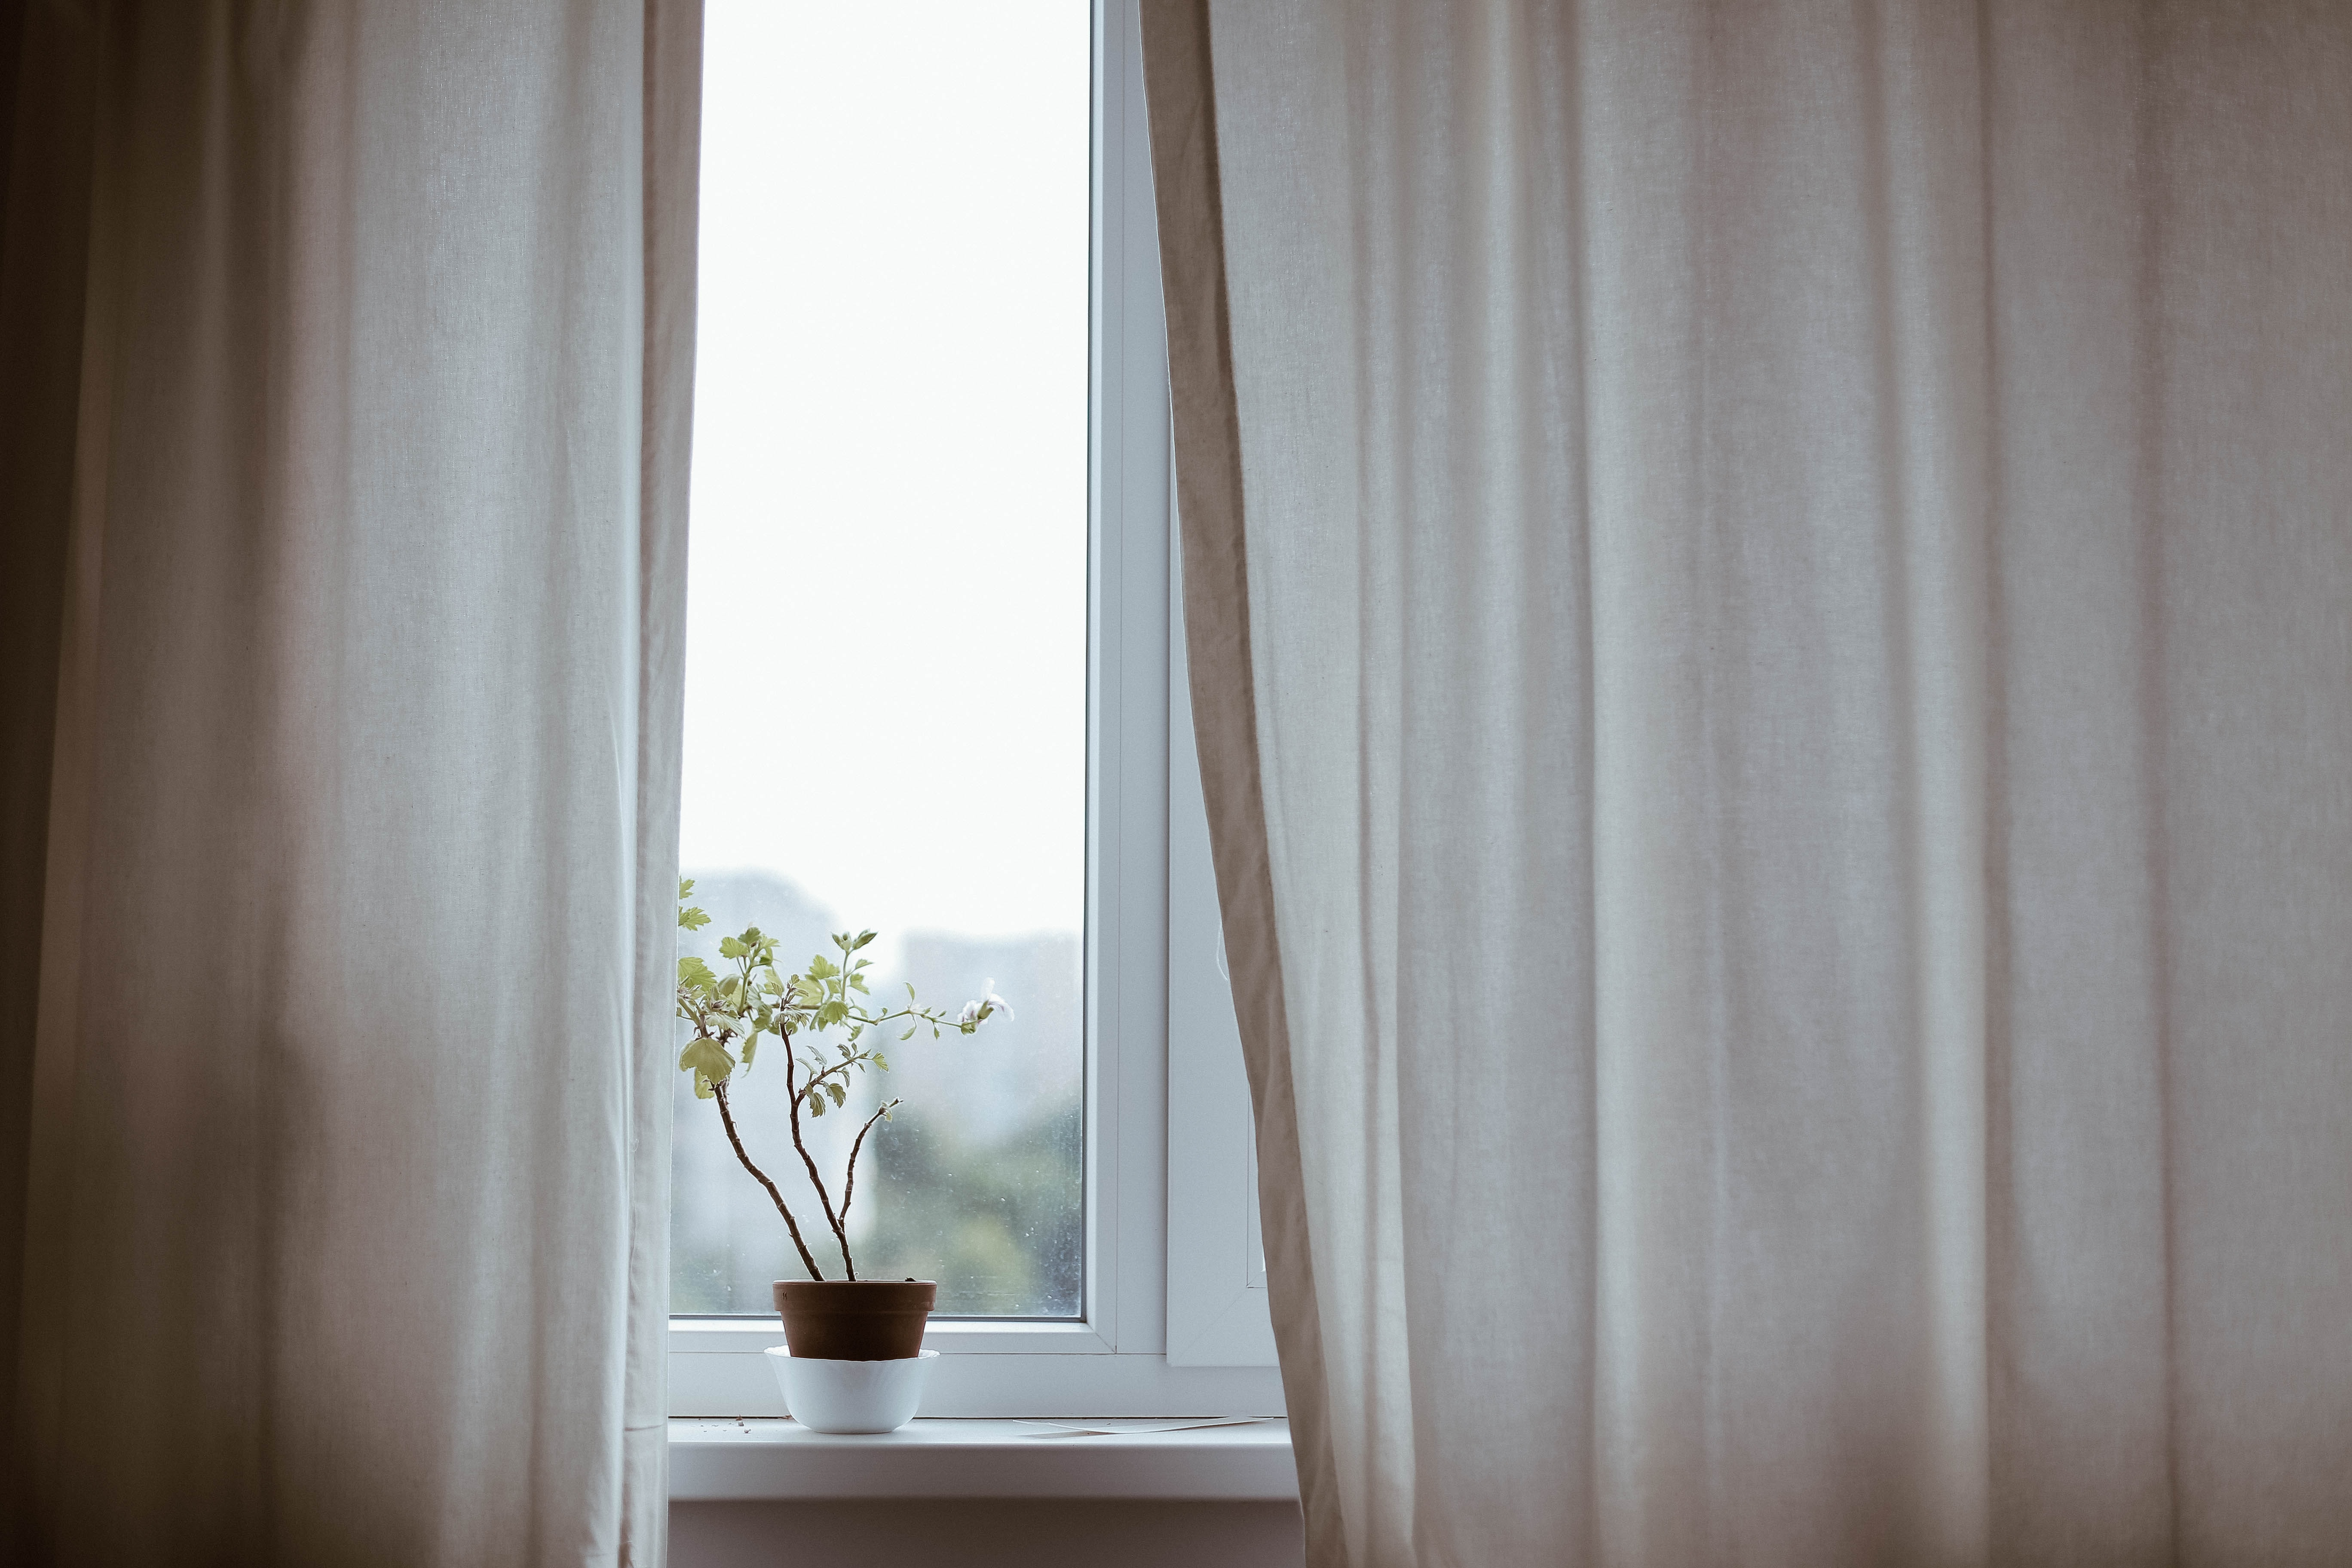
\includegraphics[width=60mm]{img/VorhangZu2}

\vspace {1.5cm}

{\fontsize{5}{6}\selectfont Photo by Eduard Militaru on Unsplash} 

% and then there was the question abt privacy
% non of the mentioned solutions seem to allow offline communication btw only the wristband and researcher laptop??
% --> this is also a point for the kids and older adults; but mainly for the ex-detainees. 

\end {frame}


%%%%%%%%%%%%%%%

%%%%%%%%%%%%%%

\begin {frame}{Open Science - at last}

Definition by FOSTER: \\

\hspace {1cm} 

Open science is the practice of science in such a way that others can \textbf{collaborate} and \textbf{contribute}, where research data, lab notes and other research processes are freely available, under terms that enable reuse, \textbf{redistribution} and \textbf{reproduction} of the research and its underlying data and \textbf{methods}.


\end {frame}


%%%%%%%%%%%%%%%

%not everyone has subscribed to OS, but for those who have, this will limit their options: 
%also, not all use cases fall necessarily under this, for example the Covid-spread-prediction 

\begin {frame}{Open Science - at last}

\begin {itemize}
\item \textbf{collaborate} and \textbf{contribute}
	\begin {itemize}
	\item collaboration on closed projects?
	\item contribution on closed projects?
	\end {itemize}
	
\item \textbf{redistribution} and \textbf{reproduction} of the research and its underlying data and \textbf{methods}

	\begin {itemize}
	\item replication of experiments based on black-box algorithms?
	\item robustness of findings between black-box algorithms?
	\end {itemize}

\end {itemize}

\end {frame}
%%%%%%%%%%%%%%%%


%Nesbitt?

%Examples of Mobile Phone studies:
%Kiukkonen, N., Blom, J., Dousse, O., Gatica-Perez, D., Laurila, J.: Towards rich mobile phone datasets: Lausanne data collection campaign. In: Proc. ACM Int. Conf. on Pervasive Services (ICPS). Berlin, Germany (2010)
%Danish study
%Sandra Servia-Rodr�guez et al. 2017. Mobile sensing at the service of mental well-being: a large-scale longitudinal study. In WWW ?17. 103?112.

%MEDEA project - The project was delayed and will start in the autumn.


%Edon project (Alzheimer UK) https://edon-initiative.org/organisation/ -- will make review of their tech choice open


%https://www.radar-ad.org
%https://radar-base.org/index.php/data-sensors/supported-devices/ -- overview of supported devices
%https://radar-base.org/index.php/project/ -- overview of projects based on Radar
%--> We tend to use these types of devices for long duration, large studies as unit cost is lower and they have proven participant acceptability, the consequence is using often propriatory processed data rather than getting raw or high resolution data data -- so it will depend on the precise nature of what you want to measure.


%http://www.tut.fi/a-wear/

%Software:
%#pre-processing, extraction of activities 
%https://github.com/wadpac/oss-dev-webinar-series-pb-field/blob/master/README.md

%#digital biomarkers
%http://dbdp.org
%https://www.cambridge.org/core/journals/journal-of-clinical-and-translational-science/article/digital-biomarker-discovery-pipeline-an-open-source-software-platform-for-the-development-of-digital-biomarkers-using-mhealth-and-wearables-data/A6696CEF138247077B470F4800090E63




\section {What are current solutions?}

%%%%%

\begin {frame}{The How }

\begin {itemize}
\item Wear OS / Android for wearables
\item Tizen for Wearables
\item astroid %- virtual machine on android OS
\end {itemize}

\end {frame}


%%%%%

\begin {frame}{The How - Android Watches}

\begin {itemize}
\item cheap-ish option 
\item https://github.com/abumondol/WaDa
	\begin {itemize}
	 \item  Accelerometer, Gyroscope, Light
  	  \item apk that can be installed offline, no accompanying phone needed
	\end {itemize}
 
\item locked into one version of the OS and the hardware that runs this one version 
 
\end {itemize}
 
 %have not tried this as yet, are there more experienced people in the room with strong feelings against this option?
 %has no license - that is an issue
  
\end {frame}

%%%%%



%%%%%

\begin {frame}{The How - Homebrew}


\center
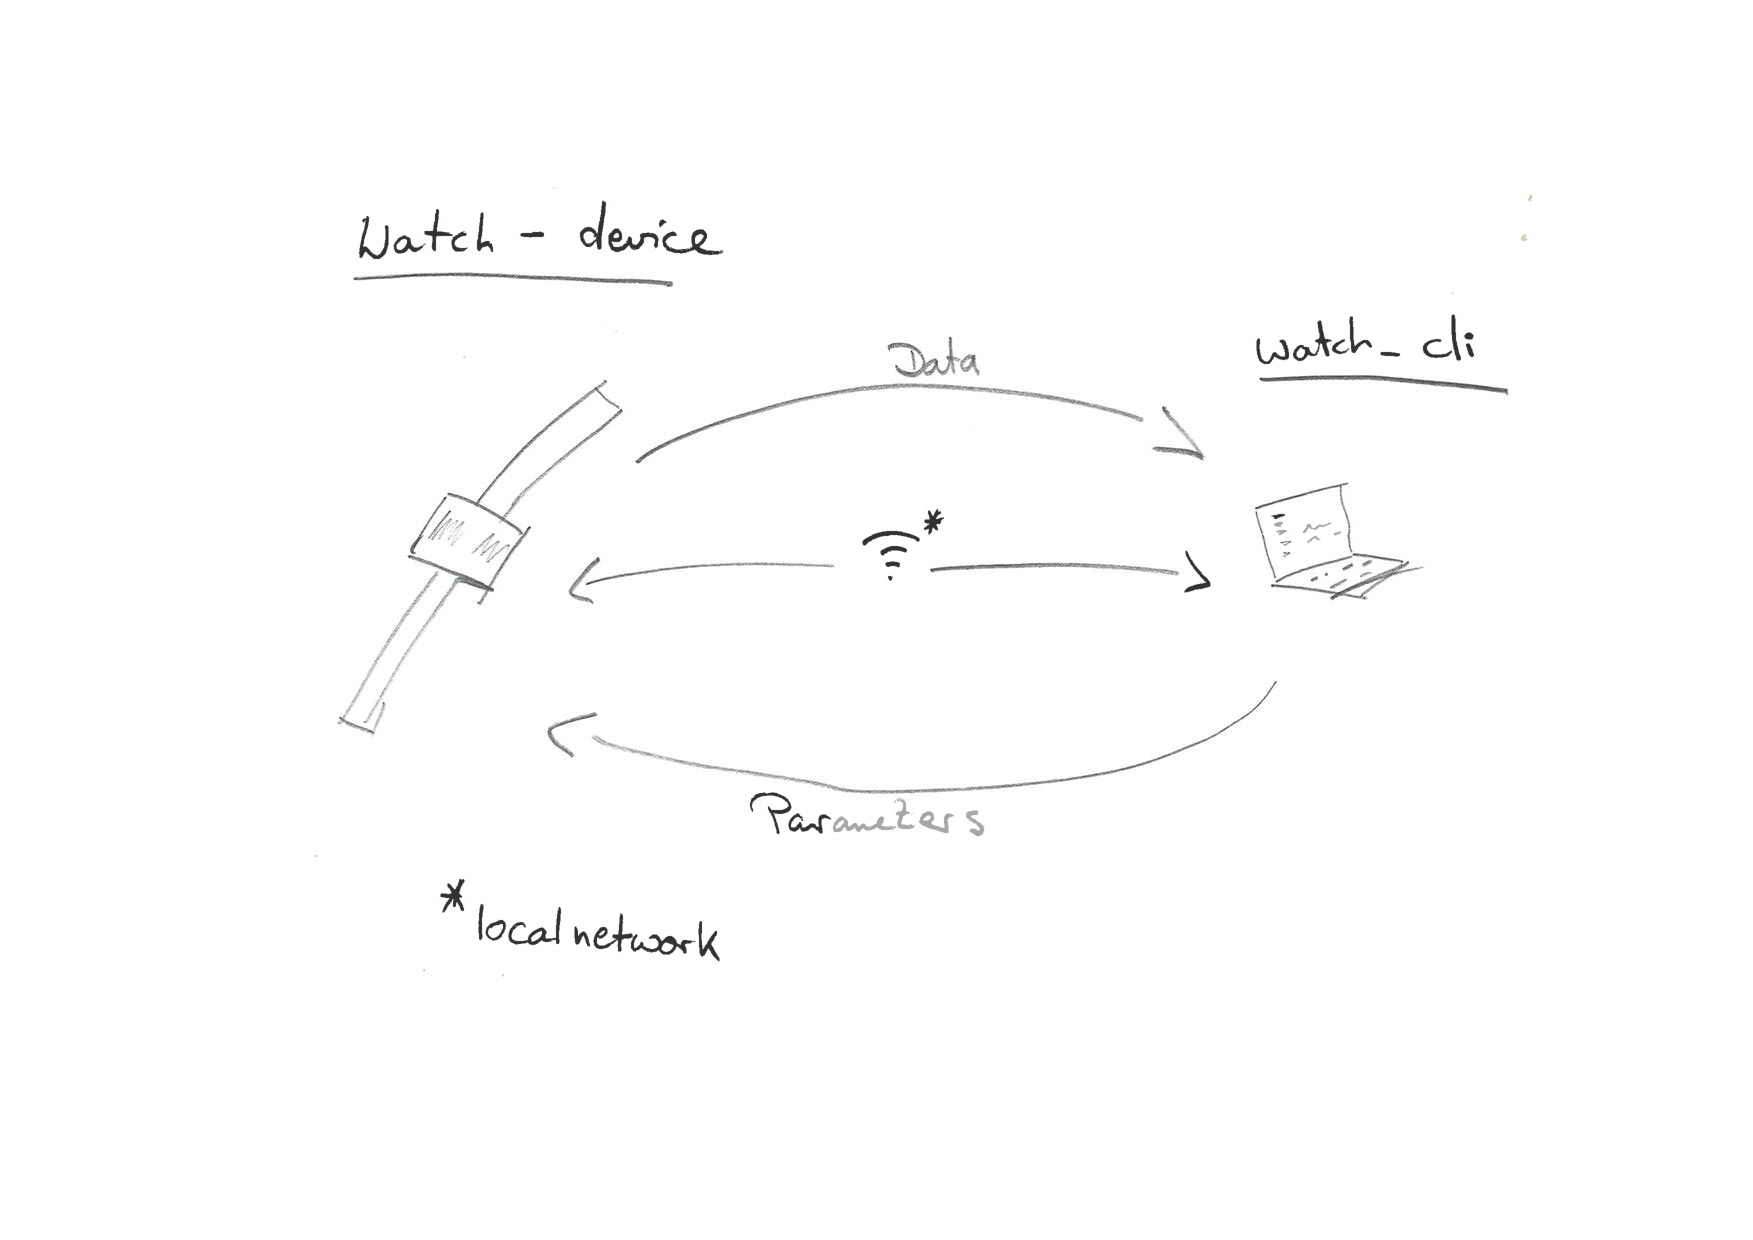
\includegraphics[width=80mm]{img/samsung}


%Watch-App for background data logging of accelerometer, gyroscope and GPS location
%CLI to set parameters for data collection

{\fontsize{5}{6}\selectfont ReadMe: https://hackmd.io/m5YRSFehSOqfGtJUXchx\_A?both } 


\end {frame}

%%%%%

\begin {frame}{The How - Homebrew}

\begin {itemize}
\item Positives	
	\begin {itemize}
	\item gets us raw data (yay, we can do DATAscience)
	\item possible to extend to: bluetooth/proximity; HR; EMA
	\end {itemize}
	\pause
			 
\item Negatives
	\begin {itemize}
	\item under construction (still....)
	\item needs good programmers 
	\item locked in to Samsung Devices 
	\end {itemize}
	
\end {itemize}

\end {frame}
%%%%%%%%


\begin {frame} {Open Source Operating System}

https://asteroidos.org/news/

%%%%%%% here is where the audience comes into play! 

\end {frame}


%%%%%

\begin {frame}{The Future }

- Data Privacy is paramount
- Research platforms allow access to some but not all data
- API's do not allow access to all data
- Interoperability 
- Robust Findings - independent of tech
- Validity of measurements
- Research questions independent of tech/ pre-trained black boxes
- Modularity to ensure only those sensors that are needed are included (and that they ARE included)
- Costs are high - open science might be an answer?
- Using big tech at exploratory research level might be fine - but where are you going with this -- access only to those who can afford it and dependent on companies to not change the modeling?
- Usually we are working towards sth - let's make sure it is in accordance with what we want to create with the tech-- also already at exploratory levels

\end {frame}


\section {What's next?}

%%%%%

\begin {frame}{The Future }
- Show design process until now - mission and network of stakeholders
- Multifaceted problem
- Difficult to get people on board, who commit and stay on board - certainly at beginning
- How do you build a OS / Open Hardware community?
- What are the benefits - especially when trying to get academics involved - incentive structure is not built for such projects

\end {frame}

%%%%%%%
\subsection {Activity: Next steps and avenues}

\begin {frame} {Wake-up Activity}
Activity with Audience: collect possible solutions to move forward
\end {frame}


\end{document}





